\documentclass[11pt,a4paper]{article}
\usepackage[latin5]{inputenc}
\usepackage[english]{babel}
\usepackage{amsmath}
\usepackage{amsfonts}
\usepackage{amssymb}
\usepackage{graphicx,subfig}
\usepackage{placeins}
\usepackage{gensymb}


\begin{document}

\section*{Report Exercise 5, Alexander Attinger \& Yannic Kilcher}

\section{Detecting interest points}
We have detected interest points with the Harris, SIFT and SURF detectors on the library and book images. We have noticed that a lot of the feature points in all detectors are around the top rims of the books as well as on the side of the books and on the writing on their covers. In Fig. \ref{fig:a11}, you can see the feature points detected with the three different detectors. We have tried to choose the parameters in a way that lead to similar results (they can be seen in our code).
We have also tried detecting keypoints on the single book images with the harris detector (Fig. \ref{fig:a12}) and have found that the detected points were in the same regions as the points in the library image.
\begin{figure}%
\centering
\subfloat[][Harris]{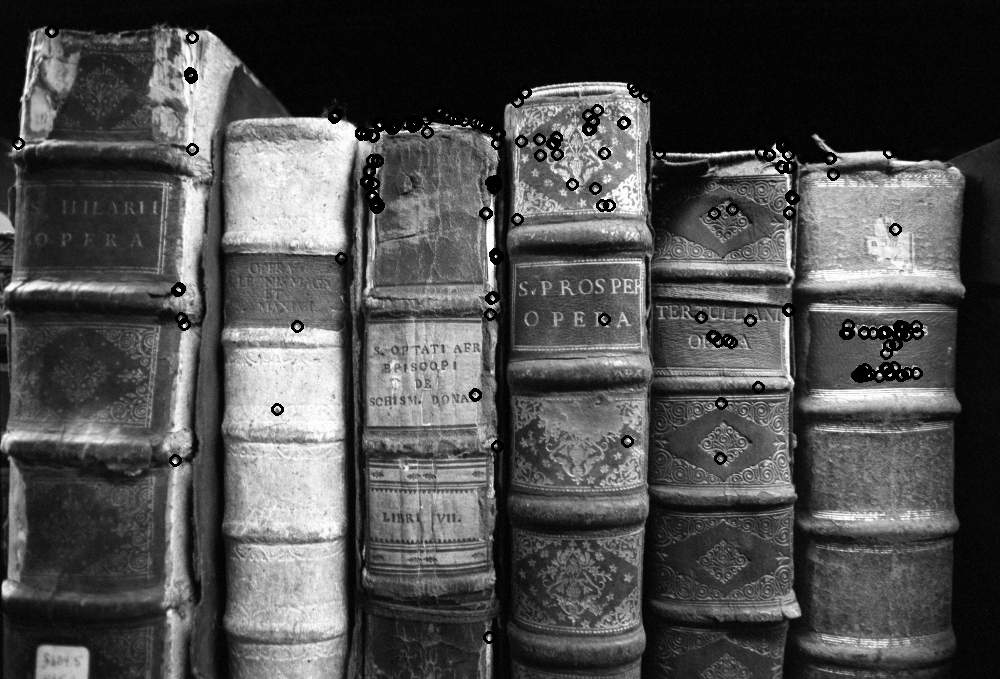
\includegraphics[scale=.3]{data/res/harris.png}}
\quad
\subfloat[][SIFT]{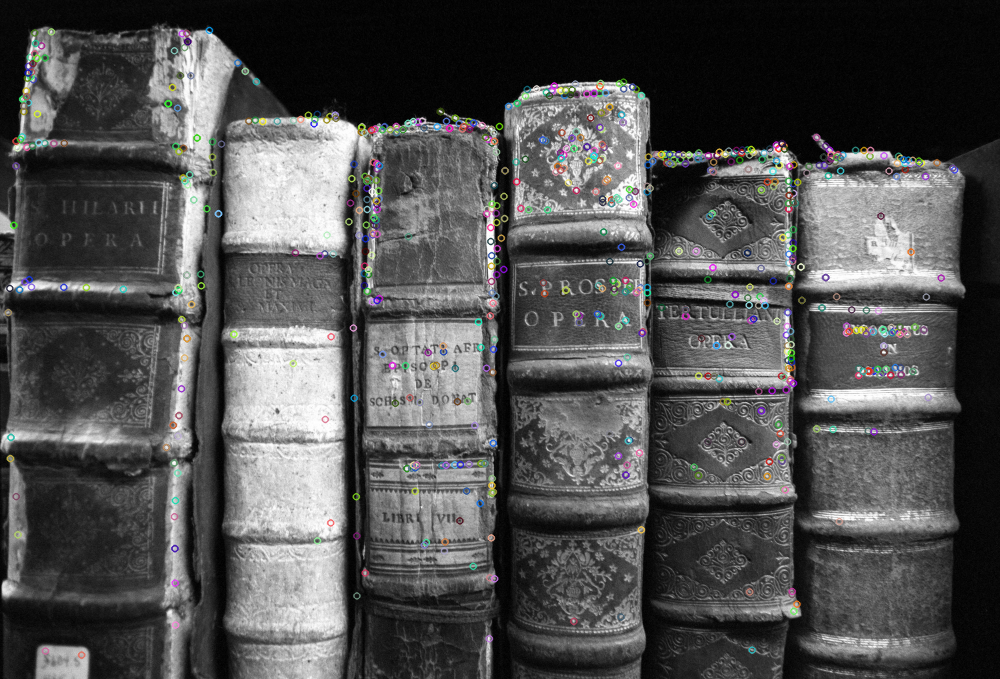
\includegraphics[scale=.3]{data/res/siftedges.png}}
\quad
\subfloat[][SURF]{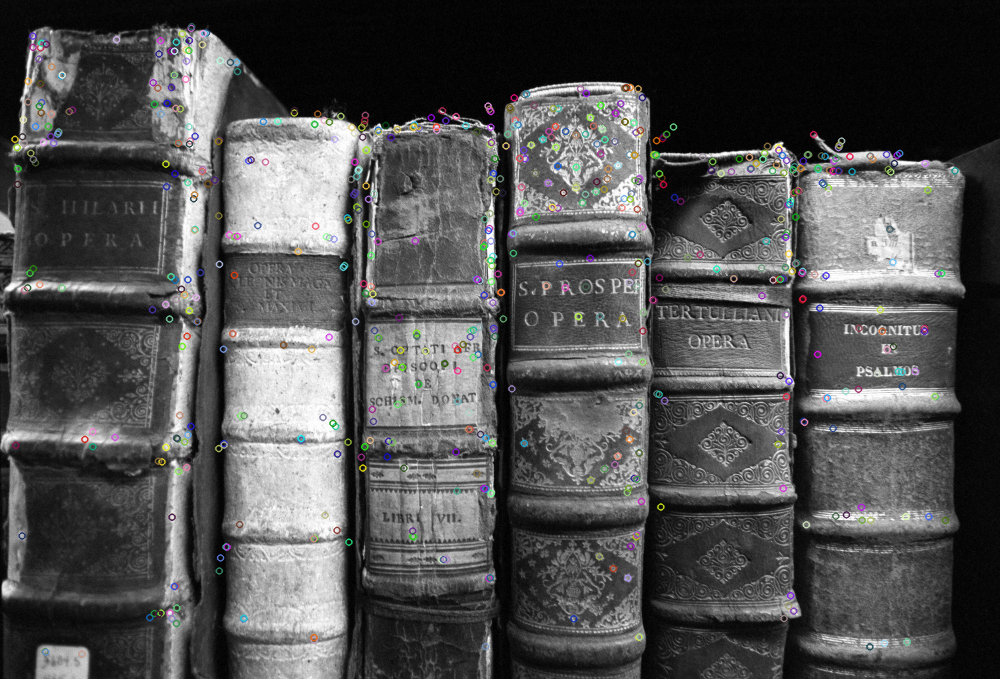
\includegraphics[scale=.3]{data/res/surfedges.png}}
\quad
\caption{Keypoint Detection}%
\label{fig:a11}%
\end{figure}
\begin{figure}%
\centering
\subfloat[][]{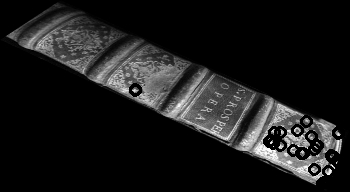
\includegraphics[scale=.3]{data/res/harris_bookp.png}}
\quad
\subfloat[][]{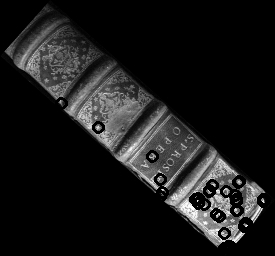
\includegraphics[scale=.3]{data/res/harris_bookr.png}}
\quad
\subfloat[][]{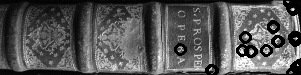
\includegraphics[scale=.3]{data/res/harris_bookt.png}}
\quad
\caption{Keypoint Detection}%
\label{fig:a12}%
\end{figure}

\FloatBarrier

\section{Matching interest points}
We have tried to detect and match keypoints on the library and book images and we have played around with different settings and thresholds for the detectors, extractors, matchers and for the filtering of matches. In Fig. \ref{fig:a21}, you can see our results where we have tried to reduce our matches so that only good matches remain. Unfortunately, we didn't get the matching for the harris detector to work as well as the SIFT and SURF, so this is the best we've gotten.
In Fig. \ref{fig:a22}, we have subtly raised the acceptance threshold for matches and we have observed that, although there are false matches, the number of correct matches also increases.
In Fig. \ref{fig:a23}, we have tried matching other book images with the library image using SURF. We had to tune the parameters from image to image in order to obtain mostly correct matches.
\begin{figure}%
\centering
\subfloat[][Harris]{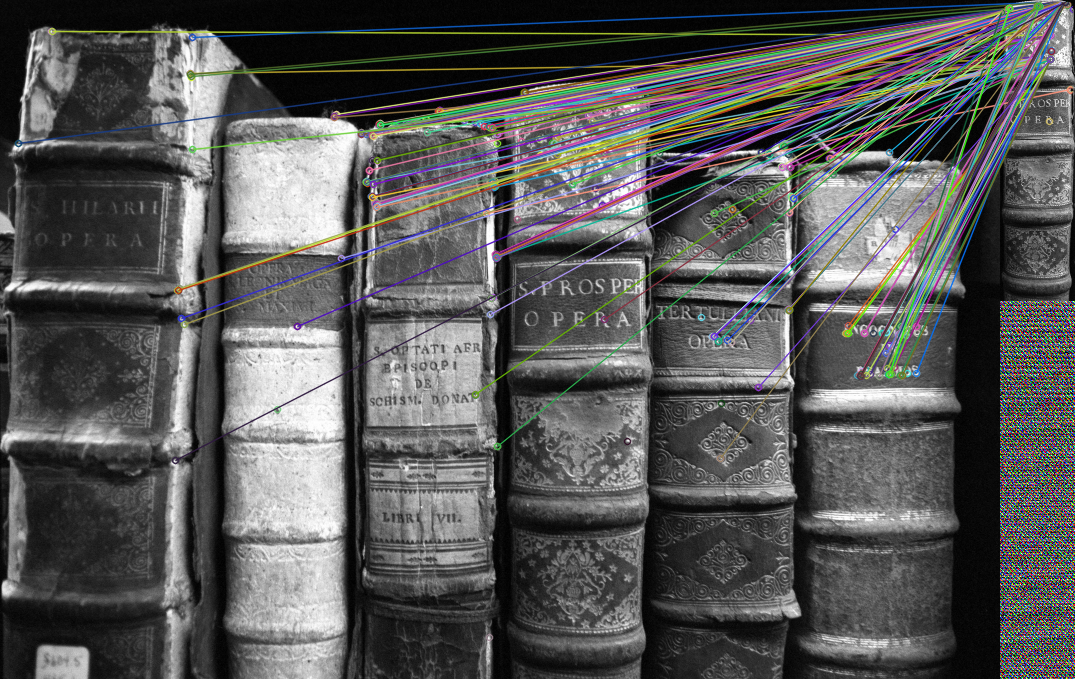
\includegraphics[scale=.3]{data/res/Matches_harris.png}}
\quad
\subfloat[][SIFT]{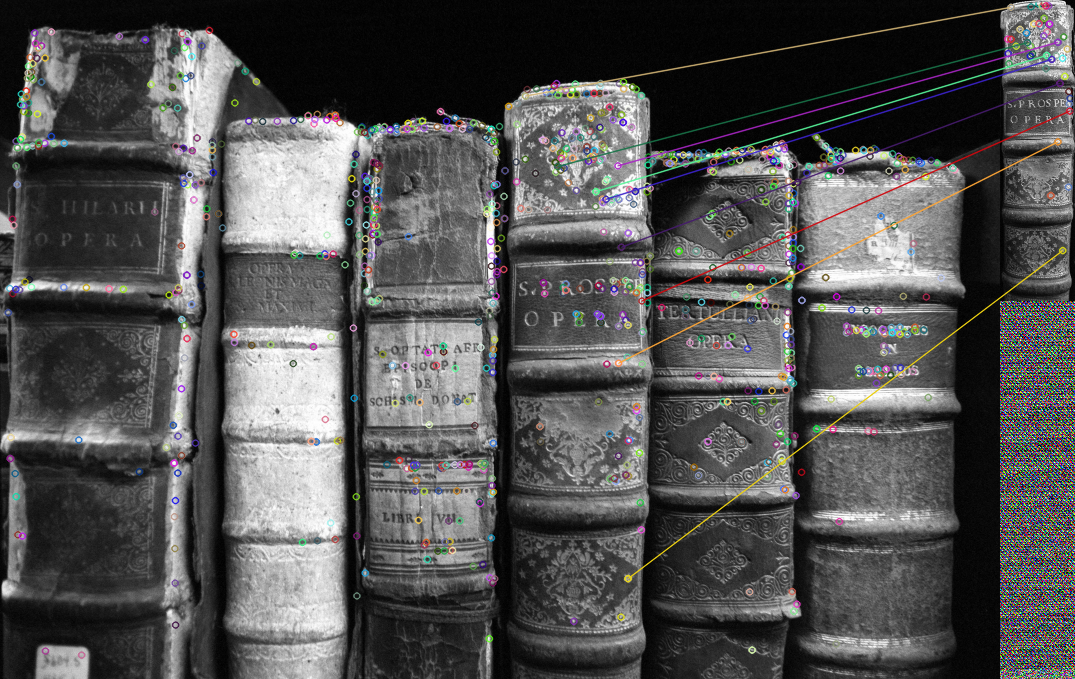
\includegraphics[scale=.3]{data/res/Matches_sift.png}}
\quad
\subfloat[][SURF]{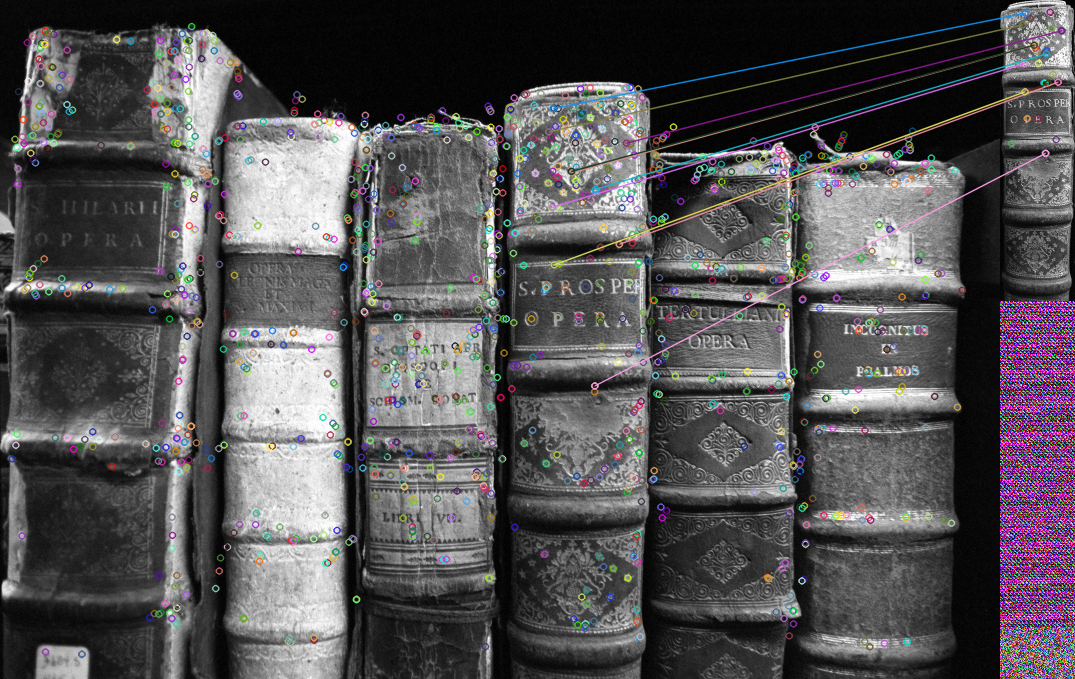
\includegraphics[scale=.3]{data/res/Matches_surf_013.png}}
\quad
\caption{Keypoint Matching}%
\label{fig:a21}%
\end{figure}
\begin{figure}%
\centering
\subfloat[][]{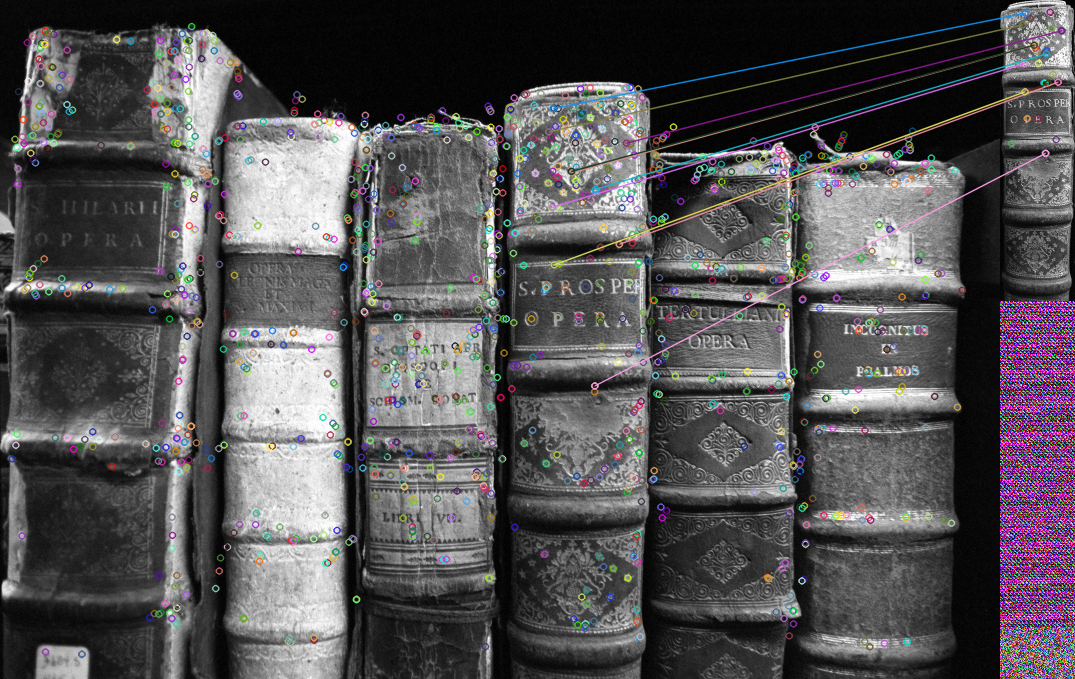
\includegraphics[scale=.3]{data/res/Matches_surf_013.png}}
\quad
\subfloat[][]{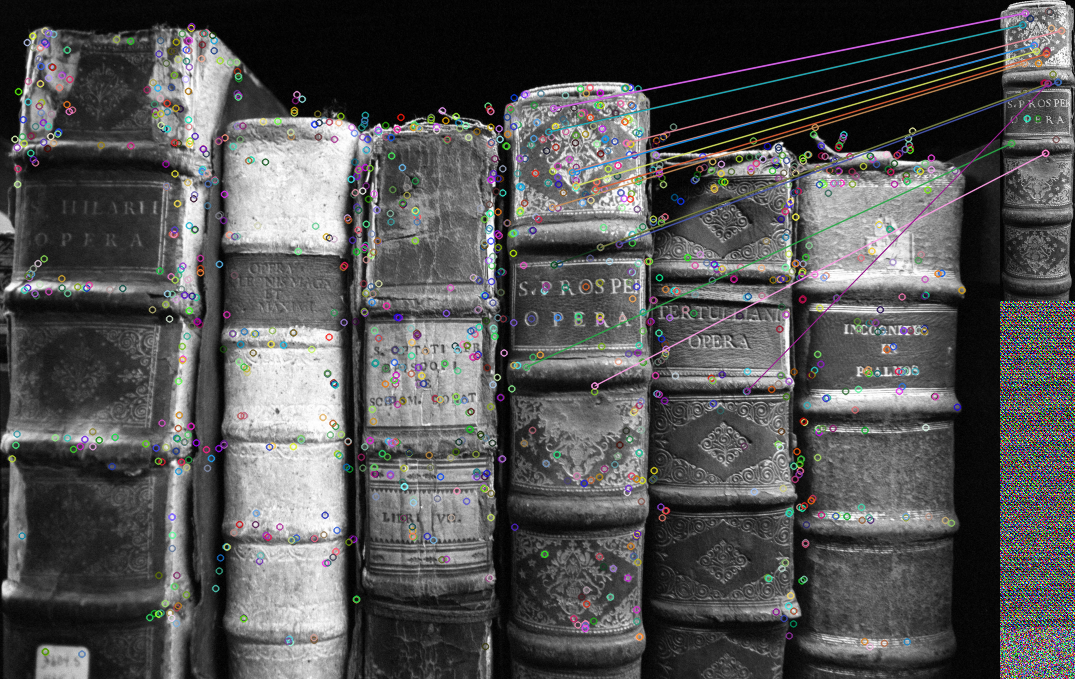
\includegraphics[scale=.3]{data/res/Matches_surf_015.png}}
\quad
\subfloat[][]{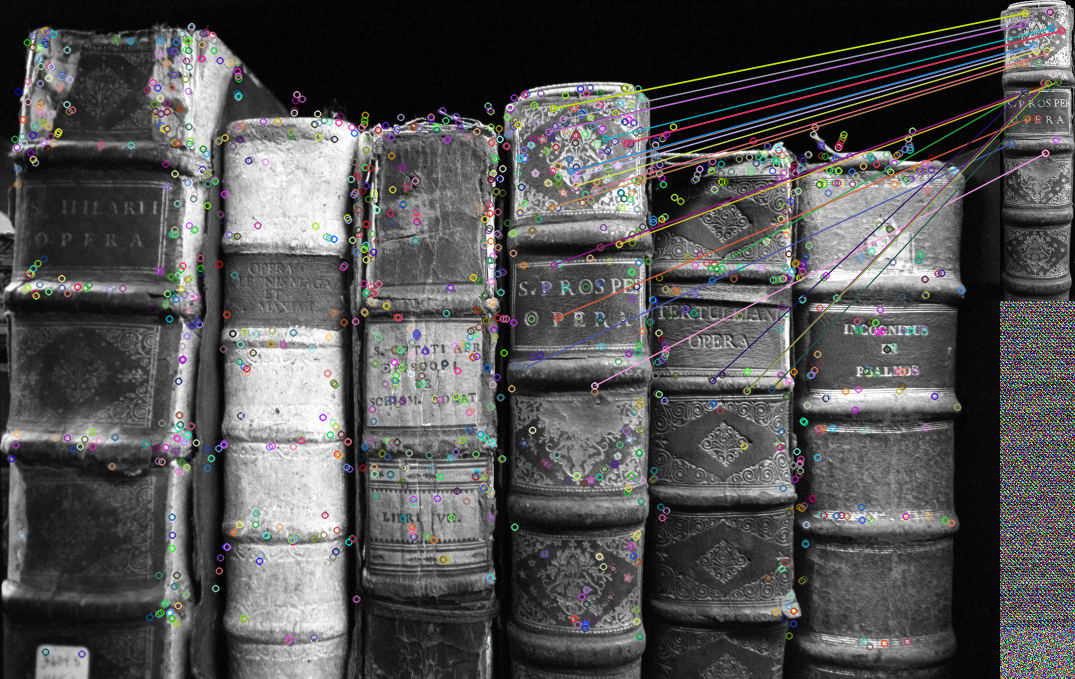
\includegraphics[scale=.3]{data/res/Matches_surf_02.png}}
\quad
\caption{Increasing thresholds on SURF}%
\label{fig:a22}%
\end{figure}
\begin{figure}%
\centering
\subfloat[][]{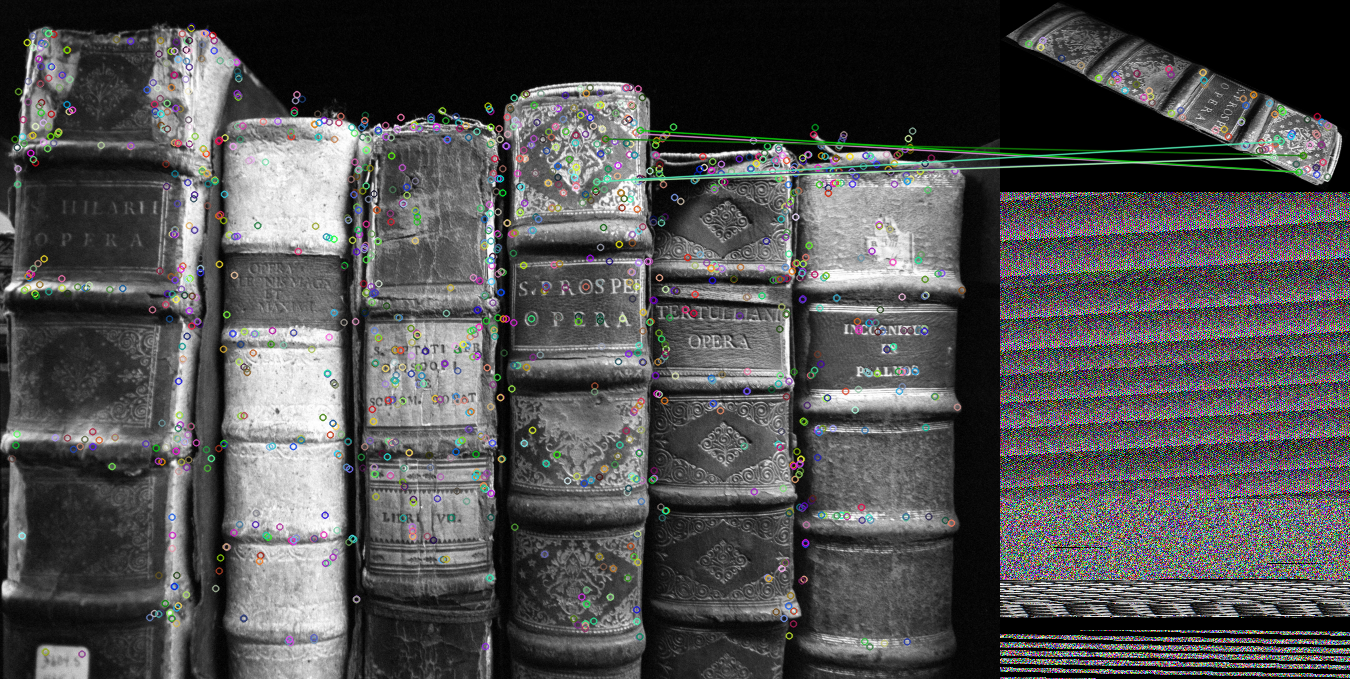
\includegraphics[scale=.3]{data/res/Matches_surfp.png}}
\quad
\subfloat[][]{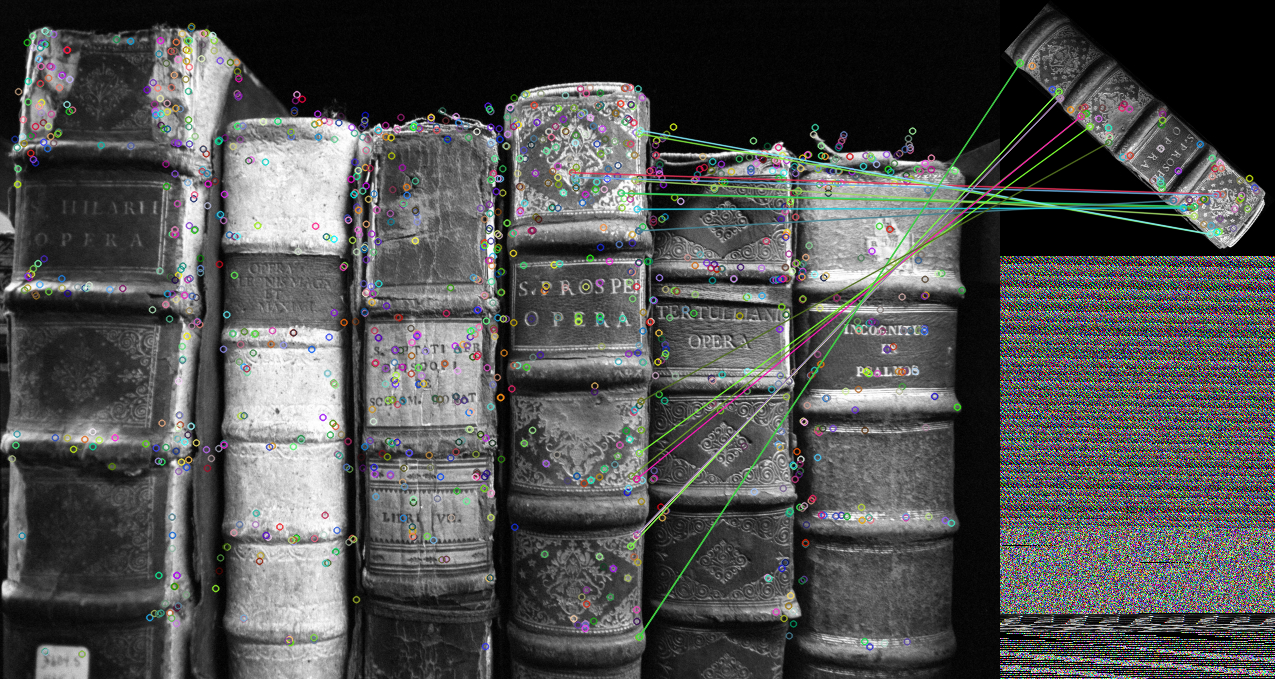
\includegraphics[scale=.3]{data/res/Matches_surfr.png}}
\quad
\subfloat[][]{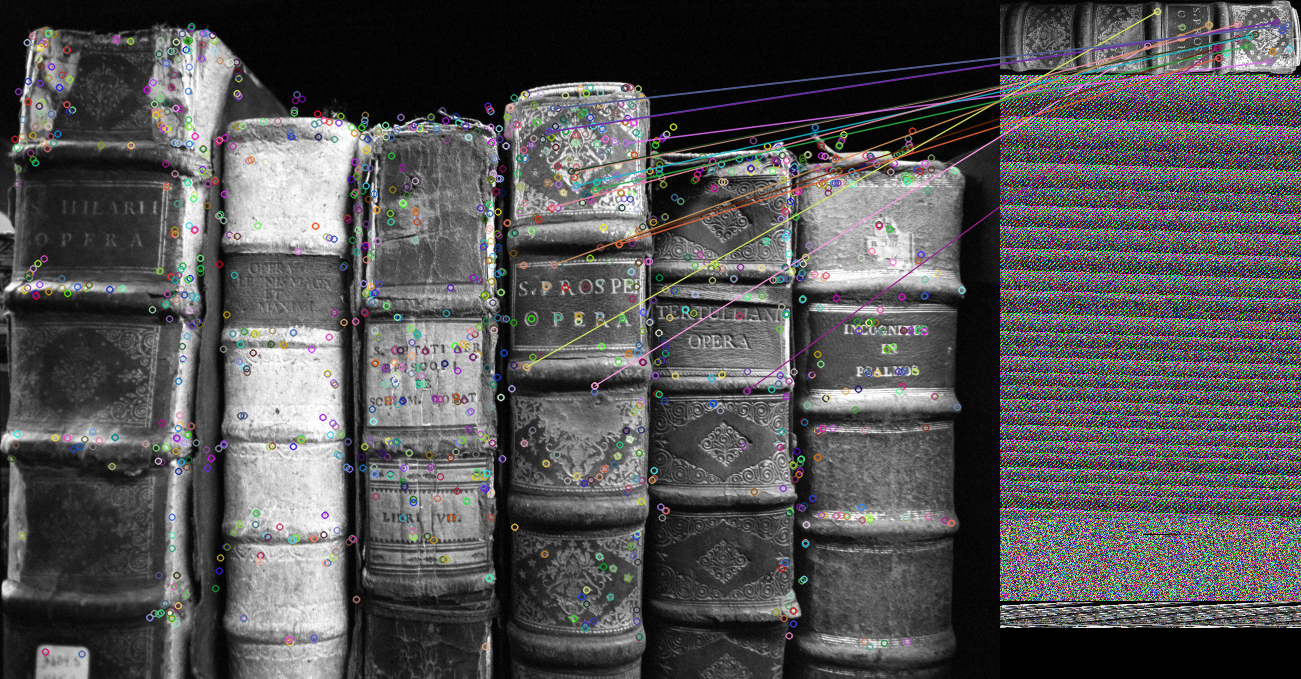
\includegraphics[scale=.3]{data/res/Matches_surft.png}}
\quad
\caption{Varying thresholds on SURF}%
\label{fig:a23}%
\end{figure}

\FloatBarrier

\section{Linefitting using RANSAC}
We have implemented the RANSAC algorithm and we have tried to fit the example data to a line using it. When constraining a to [-1,1] and b to [5,10], using an consensus ratio of 0.7 and setting the margin to 2.7, we obtain quite good results, like a = -0.775 and b = 9.643.

\end{document}
